\newcommand{\novp}{\textit{\textbf{SFNoVP}}}
\newcommand{\vp}{\textit{\textbf{SFVP}}}
\newcommand{\nfnovp}{\textit{\textbf{RRFNoVP}}}
\newcommand{\nfvp}{\textit{\textbf{RRFVP}}}

\newcommand{\optvp}{\textit{\textbf{OptVP}}}
\newcommand{\vt}{\textit{\textbf{VT}}}
\newcommand{\nfvt}{\textit{\textbf{RFVT}}}
\vspace{-1em}

This section explores how perfect branch and value predictors, paired with the new fetching scheme (RRF), improves the performance of core composition.
To understand how each component contributes to the performance improvements, different configurations were used, they are as follows:
\begin{itemize}
\item Serial fetching scheme with no value prediction (\novp).
\vspace{-1em}
\item Serial fetching scheme with perfect value prediction (\vp).
\vspace{-1em}
\item Round robin fetching scheme with no value prediction (\nfnovp).
\vspace{-1em}
\item Round robin fetching scheme with value prediction (\nfvp).
\end{itemize}

All configurations use perfect branch prediction  to ensure that core composition is always on the correct execution path.
All benchmarks are executed with 16 cores composed as this is the maximum number of cores that can be fused.
No dynamic adaptation is done as Chapter~\ref{chp:cases} showed that the primary advantage of dynamic core composition is energy savings, whereas this chapter focuses on speedup.


\subsection{Analysing the performance of the different configurations}
Figure~\ref{fig:perf_pred} shows the speedup obtained on the SD-VBS benchmarks using the different configurations.
The baseline for this section is 16 cores composed with serial fetch (SF) no value prediction (\novp) and perfect branch prediction.
This baseline is chosen as this chapter is focused on improving the performance of core composition.

First, it is clear that using RRF with value prediction (\nfvp) always results in the best speedup compared to the baseline.
For \bm{Multi\_NCut}, performance is improved by 3x when using \nfvp.
This is a significant speedup, as Chapter~\ref{chp:cases} showed that \bm{Multi\_Ncut} is a difficult benchmark for core composition (1.3x speedup in Chapter~\ref{chp:cases}).
On average, \nfvp{} outperforms the baseline by a factor of 1.88x.

\begin{figure}[t]
    \centering
    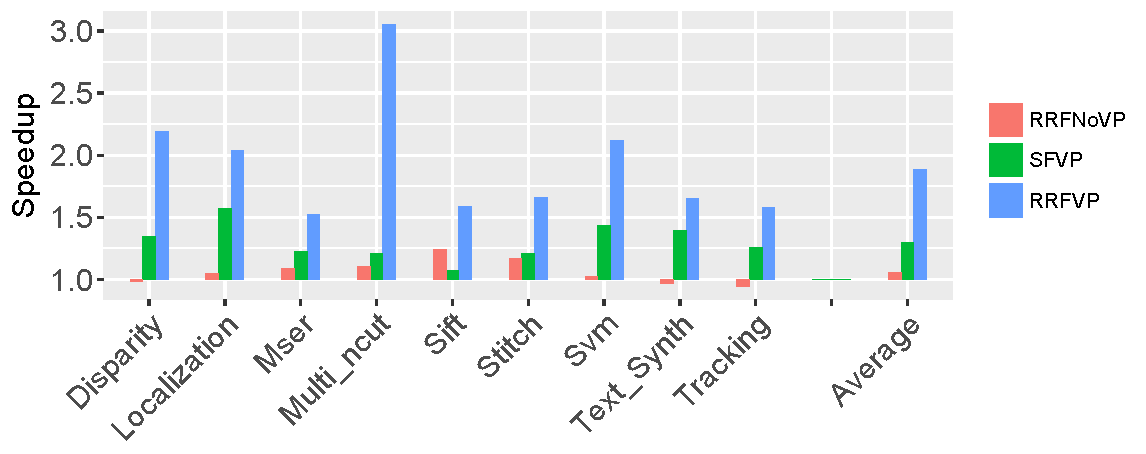
\includegraphics[width=1\textwidth]{chapter3/graphics/tempres4.pdf}
    \caption{Comparing the performance of serial fetch to round robin fetch, with and without perfect value prediction. Higher is better.}
    \label{fig:perf_pred}
\end{figure}

\subsubsection{Performance without value prediction}
The results in Figure~\ref{fig:perf_pred} show that without value prediction the performance improvements brought by RRF on its own are low, or in fact detrimental to performance.
For example, \bm{Multi\_NCut} only has a 1.10x speedup when using the \nfnovp{} configuration, compared to the 3x of \nfvp{}.
This is due to the fact that whilst more blocks are now spread across cores, the register dependencies between blocks limit the performance of the composition. 
In fact, the more even distribution is the reason why some benchmarks perform worse: \bm{Disparity}, \bm{Texture\_Synthesis} and \bm{Tracking} see a slight performance decrease.
The even distribution of blocks amongst cores increases the stress on the network on chip (NoC) as more cores will make accesses in parallel.
Without value prediction, RRF suffers due to NoC stress and data dependencies.
%In fact, \vp{} outperforms \nfnovp{} on \bm{Localization}, which shows that register dependencies between blocks can make the new fetching scheme less performant than the currently implemented.

%The performance limitations are caused by blocks that are further down the speculative path that must wait for older blocks to write to the register file.


\subsubsection{Performance with value prediction}
The performance improvements brought by RRF are more apparent when taking value prediction into account.
\nfvp{} has a 54\% performance increase compared to \vp{} (1.88x vs 1.22x).
The difference in performance comes from the fact that with value prediction, blocks can potentially execute faster, and thus a faster fetching scheme is required to keep up.
Since the SF scheme is slower, it is less likely going to benefit from parallel execution.
Even so, \vp{} results in a 1.5x speedup for \bm{Localization} which shows that value prediction is valuable for composition regardless of the scheme.

\begin{figure}[t]
    \centering
    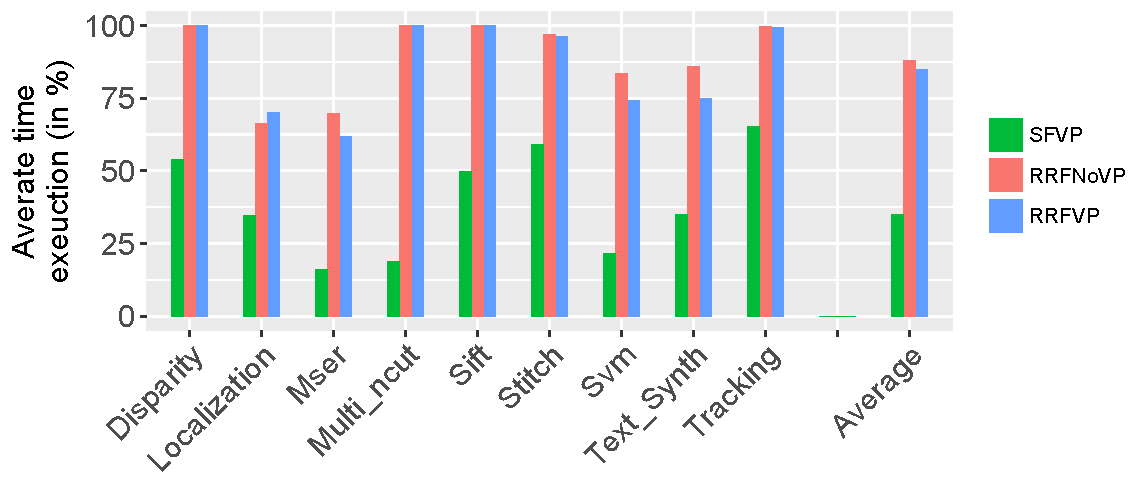
\includegraphics[width=1\textwidth]{chapter3/graphics/perf_av_cycle_exec4.pdf}
    \caption{Average time each core is executing blocks (in \%) for each benchmark, using the different configurations. Higher is better.}
    \label{fig:perf_av_cycle}
	\vspace{1em}
\end{figure}

\paragraph*{Active Cycles}
To better highlight how the SF scheme hinders performance even with value prediction, the percentage of time a core in a composition is actively executing code, for each benchmark, is shown in Figure~\ref{fig:perf_av_cycle}.
For each configuration, the number of cycles each core in a composition has instructions to execute is averaged out and then compared to the total execution time of the application.
When the average active time of a core is close to the total execution time, this means that the composition was efficiently used, as each core had a block to run throughout the program execution.

Figure~\ref{fig:perf_av_cycle} shows that \vp{} often has low active times when using a composition of 16 cores.
This is due to the fact that the SF scheme is slow, and thus, some cores are inactive, waiting to receive a fetch request from another core.
The lower the percentage is, the less likely there are going to be multiple blocks on different cores in flight which in turn means the composition is less efficient and value prediction is less useful.
Since value prediction is aimed at increasing instruction level parallelism (ILP)~\cite{peraisBeBop2015} it is important that cores may fetch blocks quickly in a composition.

%Of course, it is important to note that their LSQs and L1 caches may still be used by other active cores, simply that their execution units are not being used.


With the RRF scheme, the percentage of active time is increased on average by a factor of 2.28x, and is on average 85\%.
This means that during most of the execution of an application, all cores are executing code, and thus greatly increases the chance of improving performance via core composition.
It is interesting to see that \nfvp{} has a lower average time than \nfnovp{} for some benchmarks such as \bm{MSER} and \bm{Texture\_Synthesis}.
Also, whilst RRF aims to evenly distribute blocks amongst the cores, the average core utilisation for \bm{Localization} with the configurations \nfnovp{} and \nfvp{} is of 62\%.
This reduced average time is due to flushes caused by Load-Store-Queue (LSQ) violations, which causes cores to flush their instruction windows, and thus increases the number of times that cores will not be executing code.
Figure~\ref{fig:lsqvio} shows the number of blocks that cause an LSQ violation, normalised by the number of fetched blocks for each of the benchmarks.
Even though the percentage of violations is small, it still has an impact on how efficient the composition is, due to the fact that compositions rely on heavy speculation to obtain any performance improvements.
\begin{figure}[t]
    \centering
    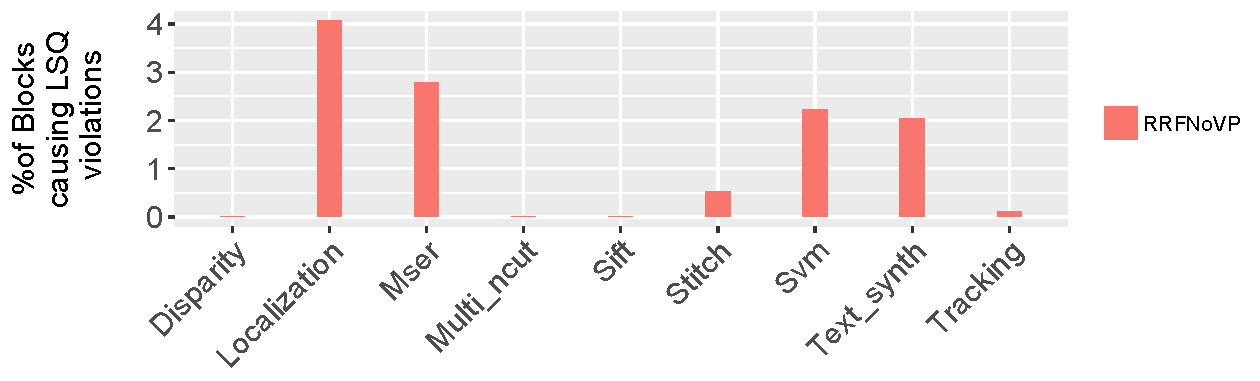
\includegraphics[width=1\textwidth]{chapter3/graphics/lsqViol4.pdf}
    \caption{Number of blocks that cause LSQ violations, normalised by the number of fetched blocks for each of the benchmarks.}
    \label{fig:lsqvio}
	\vspace{1em}
\end{figure}

%A store-set dependency predictor is implemented in the processor~\cite{chrysos1998storesets}, however it is sometimes hard to predict load-store dependencies across multiple blocks, which is why LSQ violations occur.
%Store-set dependency predictors are not discussed in more detail in this chapter, however researching how store-set dependencies could be applied to core-composition is an interesting subject for future work.


\subsubsection{Summary}

This section shows that a perfect branch predictor, paired with perfect value prediction and the round robin fetching scheme can outperform the current configuration by a factor of up to 3x and on average a speedup of 1.87x.%, and can potentially be improved to 2.35x with further modifications to the fetching scheme.
This section also showed that without value prediction RRF only obtains a 1.09x speedup compared to the serial fetching scheme.
This is due to the fact that the benchmarks all display a certain amount of data-dependencies between blocks and that spreading blocks across cores more evenly can put pressure on the NoC; thus reduce the performance improvements of fetching blocks quicker.

